\subsubsection{Prvo, pa 1}

\def\fibonacci#1#2#3{%
\newcount\a \a=#1
\newcount\b \b=#2
\number\a,~\number\b
\newcount\t
\newcount\n \n=#3 \advance\n-2
\loop
  \t=\b \advance\b\a \a=\t
  , \number\b
  \advance\n-1
\ifnum \n>0 \repeat}

\zadatak 
Koliki procenat cena {\sl od igle do lokomotive\/}
% Koliki procenat {\sl Fibona{\cv}ijevih brojeva\/} (Leonardo Bonacci) \fibonacci11{25},~\dots\
po{\cv}i{\nj}e cifrom~1?

\resenje Iz formule \eqref{eq:benford} sa strane \pageref{eq:benford} sledi da je $P(10,1)=\logten 2 \approx \ram{30\%}$.

\dodatak Ovu zakonitost je prvi otkrio 1881.\ astronom {\Nj}ucom (Simon Newcomb), kada je primetio da su
listovi logaritamskih tablica koje je dugo koristio najpr{\lj}aviji
na po{\cv}etku: \smash{\hbox{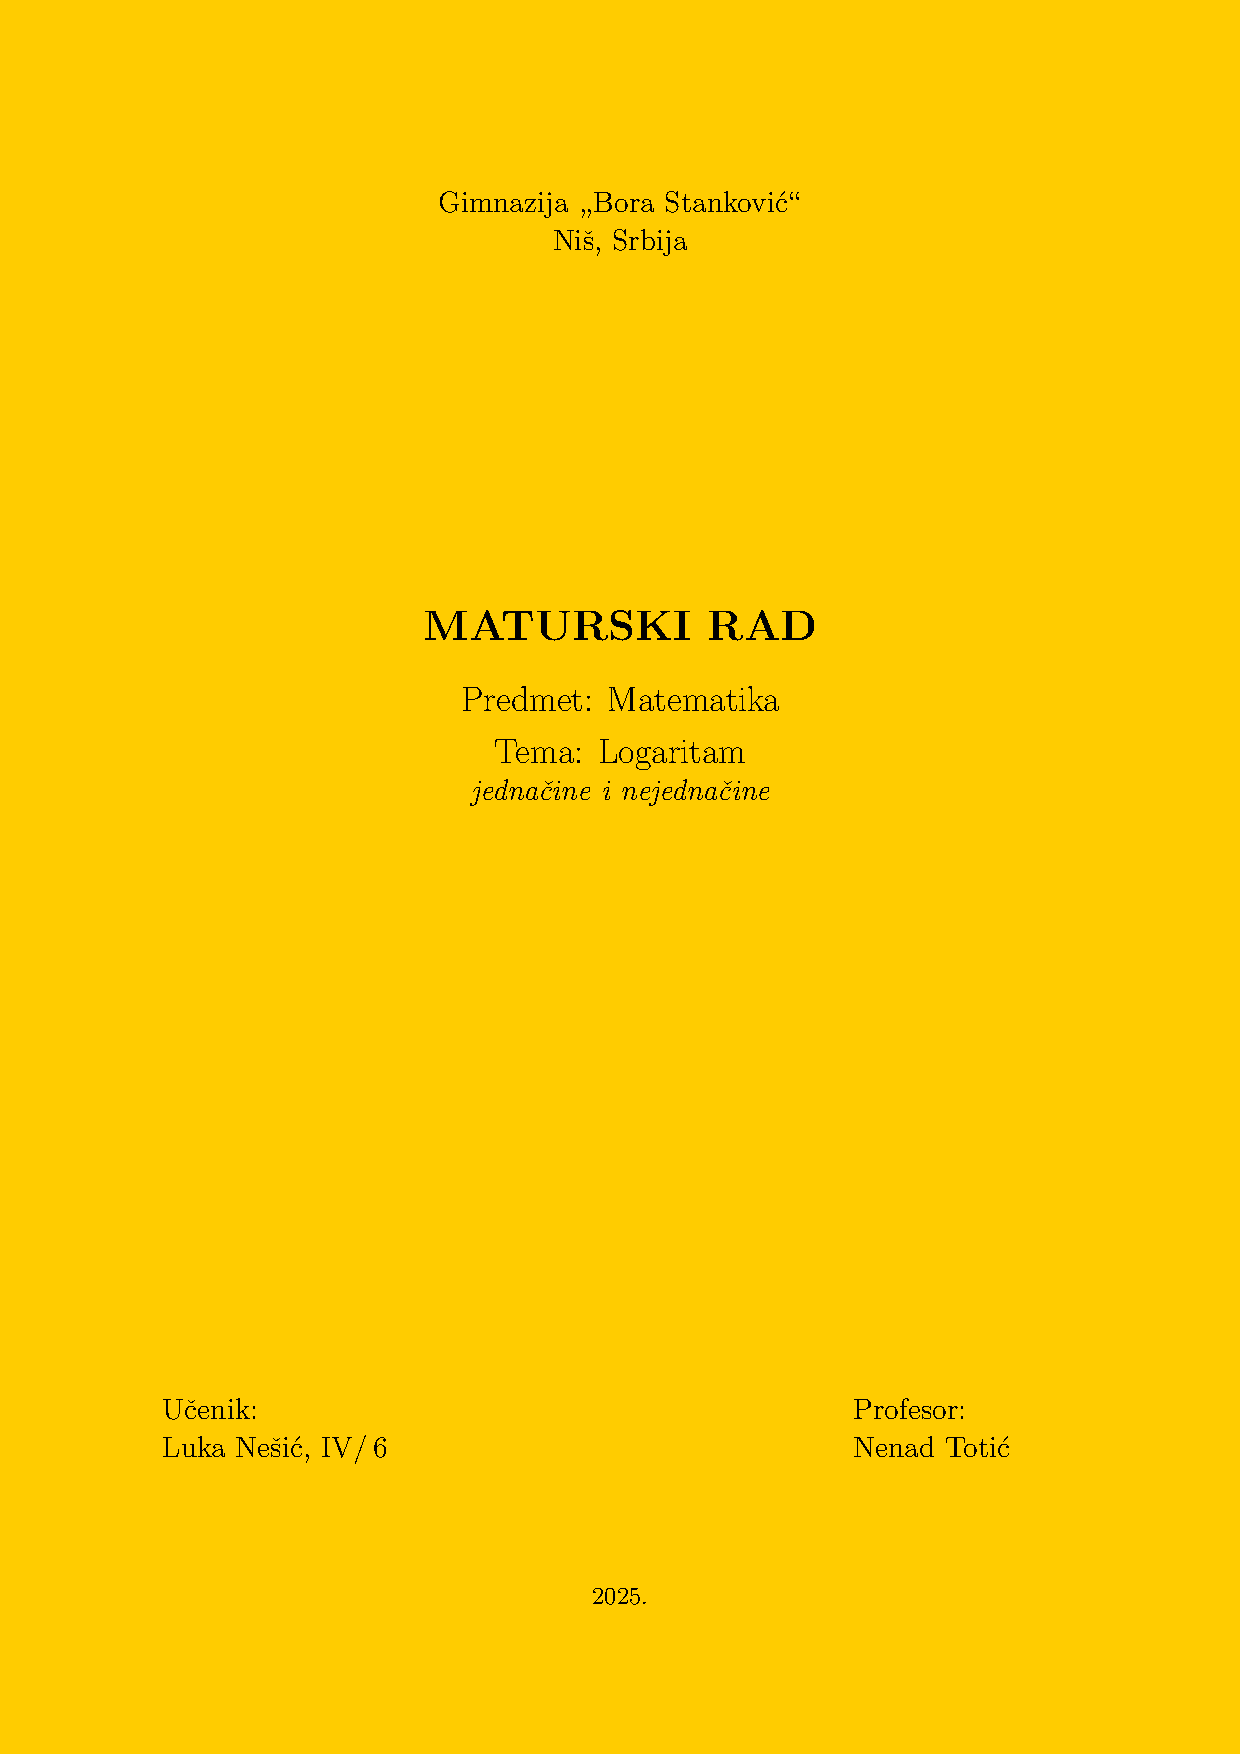
\includegraphics{log.4}}}.
U filmu {\sl Ra{\cv}unovo{\dj}a\/} ({\sl The Accoutant\/}), glavni lik (Ben Afflec) otkriva
da su finansijski izve{\sv}taji preprav{\lj}ani jer uvi{\dj}a da
ne prate ovo pravilo.